\documentclass{article}
\usepackage[utf8]{inputenc}
\usepackage[T1]{fontenc}
\usepackage[spanish]{babel}
\usepackage[hidelinks]{hyperref}
\usepackage{graphicx}
\usepackage{titling}
\usepackage{float}
\usepackage{longtable}
\usepackage[text={18cm,21cm},centering]{geometry}
\usepackage{hyperref} \hypersetup{ colorlinks=true, linkcolor=blue, filecolor=magenta,
urlcolor=blue, }
\usepackage{listings}
\usepackage{xcolor}
\usepackage{booktabs}



% Definir colores adicionales si es necesario
\definecolor{gray}{rgb}{0.5, 0.5, 0.5}
\definecolor{lightgray}{rgb}{0.9, 0.9, 0.9}
\definecolor{green}{rgb}{0, 0.5, 0}
\definecolor{blue}{rgb}{0, 0, 1}
\definecolor{red}{rgb}{1, 0, 0}

\lstdefinestyle{mystyle}{
    backgroundcolor=\color{white},   
    commentstyle=\color{green},
    keywordstyle=\color{blue},
    numberstyle=\tiny\color{gray},
    stringstyle=\color{red},
    basicstyle=\ttfamily\footnotesize,
    breakatwhitespace=false,         
    breaklines=true,                 
    captionpos=b,                    
    keepspaces=true,                 
    numbers=left,                    
    numbersep=5pt,                  
    showspaces=false,                
    showstringspaces=false,
    showtabs=false,                  
    tabsize=2
}

\lstset{style=mystyle}


\begin{document}


\begin{titlepage}
    \centering
    {\bfseries\LARGE Universidad de La Habana \par}
    \vspace{1cm}
    {\scshape\Large Facultad de Matemática y Computación \par}
    \vspace{3cm}
    {\scshape\Huge Predicción de Problemas de Codeforces\par}
    \vfill
    
    {\Large Juan Carlos Espinosa Delgado C-411 \par}
    {\Large Raudel Alejandro Gómez Molina C-411 \par}
    {\Large Alex Sierra Alcalá C-411 \par}
    {\Large Yoan René Ramos Corrales C-412 \par}
    \vfill
    {\href{https://github.com/ARJ-Code/codeforce-tag-predictor}{Proyecto en github} \par}
\end{titlepage}

\section{Introducción}

\subsection{Motivación}

La plataforma Codeforces es una herramienta fundamental en la comunidad de programación competitiva, diseñada
para desarrollar y entrenar habilidades de resolución de problemas. Los problemas en Codeforces no solo desafían
a los competidores, sino que también proporcionan una base sólida para aprender y aplicar diversos algoritmos y
estructuras de datos. Cada problema está asociado a una serie de categorías o etiquetas que ayudan a identificar
los tipos de algoritmos y técnicas necesarias para resolverlos. Pero este proceso suele estar muy apegado a la
a la solución final del ejercicio por lo que la correcta identificación de los tags suele ser un gran reto para los
competidores.

Es válido aclarar que la automatización de este proceso no es interés de la programación competitiva, ya que en estos
escenarios lo que se busca es el razonamiento lógico de los competidores, en este contexto si pudiera ser interesante
el desarrollo de un mecanismo de generación de problemas, pero este no es el objetivo de este proyecto.

Sin embargo la experimentación con la detección de tags en escenarios controlados como este, manteniéndonos en el entorno
de que esta tarea es útil para la posterior solución del problema pudiera servir de base para proponer mecanismo de detección
de tags en problemas reales orientados al campo de la generación de algoritmos.

\subsection{Problemática}

Cada problema en la plataforma Codeforces y un problema de programación competitiva en general cuenta primeramente con
un título y una descripción en la cual se plantea el objetivo y la problemática del mismo, este segundo componente del
problema es la principal fuente de interés para la detección de tags ya que estos se encuentran explícitos en forma de
lenguaje natural en dicha descripción.

Pero además de la descripción los problemas cuentan con una restricción de tiempo y espacio de memoria donde se deben
desenvolver los algoritmos que den solución al problema (un algoritmo correcto para todos los casos de prueba
que no este dentro de los límites establecidos no es considerado como solución). Ahora bien esta restricción también
influye en los tags del algoritmo ya el conjunto de tags del problema que satisfacen estas restricciones y la descripción
del problema será subconjunto del conjunto de tags solo asociados a la descripción.

Otra característica interesante que nos pudiera aportar información sobre la naturaleza del problema es analizar el
código de una solución aceptada del problema, ya que es posible identificar los tags asociados a dicho código y por
tanto un subconjunto de los tags del problema. Es importante analizar que con este enfoque solo podemos obtener un
subconjunto de los tags ya que un mismo problema puede tener multiples soluciones y cada solución puede tener asociada
distintos tipos de tags.

Por tanto como tenemos de por medio un problema asociado a lenguaje natural y actualmente no hay ningún método asociado
medianamente eficaz asociado a este campo que no lleve Machine Learning, la propuesta de la solución descrita en este
trabajo empleará algoritmos de Machine Learning los cuales iremos introduciendo a lo largo de este trabajo.

\subsection{Objetivos Generales y Específicos}

\subsubsection{Objetivos Generales}

El objetivo general de este proyecto es desarrollar un sistema automatizado utilizando técnicas de Machine Learning para detectar y asignar etiquetas (tags) a los problemas de programación en Codeforces.


\subsubsection{Objetivos Específicos}

\begin{itemize}
    \item \textbf{Recolección y Preprocesamiento de Datos:}
          \begin{itemize}
              \item Recolectar un conjunto representativo de problemas de Codeforces, incluyendo sus descripciones, restricciones de tiempo y memoria, y etiquetas existentes.
              \item Realizar el preprocesamiento del texto de las descripciones para normalizar y limpiar los datos, facilitando su análisis.
          \end{itemize}
          
    \item \textbf{Desarrollo del Modelo de Machine Learning:}
          \begin{itemize}
              \item Investigar y seleccionar algoritmos de Machine Learning apropiados para la tarea de clasificación de texto, como KNN, Naive Bayes, y redes neuronales.
              \item Entrenar varios modelos utilizando el conjunto de datos preprocesado, ajustando hiperparámetros para optimizar el rendimiento.
          \end{itemize}
          
    \item \textbf{Evaluación del Modelo:}
          \begin{itemize}
              \item Evaluar los modelos entrenados utilizando métricas de rendimiento como precisión, recall, F1-score y exactitud.
              \item Comparar los resultados de diferentes modelos para identificar el más eficaz en la detección de etiquetas.
              \item Comparar los resultados con un modelo de lenguaje (en este caso se usará Chat-GPT 3.5).
          \end{itemize}
          
    \item \textbf{Implementación y Prueba:}
          \begin{itemize}
              \item Implementar el modelo seleccionado en un entorno de prueba para evaluar su rendimiento en condiciones reales.
              \item Realizar pruebas adicionales para validar la consistencia y robustez del sistema en la asignación de etiquetas.
          \end{itemize}
          
    \item \textbf{Documentación y Propuesta de Mejora:}
          \begin{itemize}
              \item Documentar el proceso completo de desarrollo, incluyendo la recolección de datos, preprocesamiento, desarrollo del modelo, evaluación e implementación.
              \item Proponer mejoras y futuras líneas de investigación basadas en los resultados obtenidos y las limitaciones encontradas durante el desarrollo del proyecto.
          \end{itemize}
\end{itemize}

\subsubsection{Hipótesis}

\begin{itemize}
    \item \textbf{Hipótesis Principal:} Un modelo de Machine Learning bien entrenado puede detectar y asignar etiquetas (tags) a los problemas de programación de Codeforces con una precisión comparable a la de un humano experto.
    \item \textbf{Hipótesis Secundarias:}
          \begin{itemize}
              \item Los algoritmos de clasificación de texto basados en redes neuronales (como LSTM o Transformers) ofrecerán un mejor rendimiento en la detección de etiquetas en comparación con algoritmos más tradicionales como Naive Bayes o KNN.
              \item El análisis y utilización de las restricciones de tiempo y memoria, así como del código de soluciones aceptadas, pueden mejorar significativamente la precisión del modelo en la asignación de etiquetas.
          \end{itemize}
\end{itemize}

\section{Análisis de los datos}

Como dataset usaremos un conjunto de problemas de Codeforces con su identificador, descripción, conjunto de tags, puntos y rating. 

\subsection{Exploración de datos}

Para esto primero exploramos los datos buscando filas con ausencia de datos y eliminamos datos que no son de interés para
nuestro problema. 

En este caso hemos identificado que las columnas asociadas a los puntos y el rating cuentan con valores neuronales
y no representan interés para nuestro problema por lo que hemos decidido eliminarlas.

Luego analizamos el contenido de la descripción de los problemas y identificamos el idioma de las mismas ya que esta
información puede ser útil para el futuro análisis empleando modelos de lenguaje.

\subsubsection{Información recopilada sobre los datos}

\begin{itemize}
    \item Distribución de la longitud del texto de los Problemas
          \begin{center}
              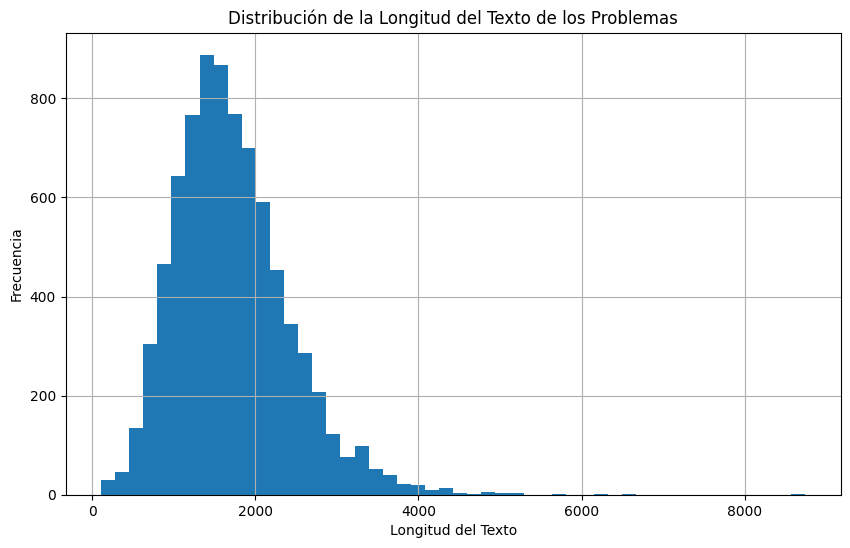
\includegraphics[scale=0.8]{imgs/len_description.png}
          \end{center}
          en la gráfica anterior se puede observar que la longitud de los problemas que más abunda sobre los 2000 caracteres.
          \newpage          
    \item Frecuencia de las etiquetas más comunes
          \begin{center}
              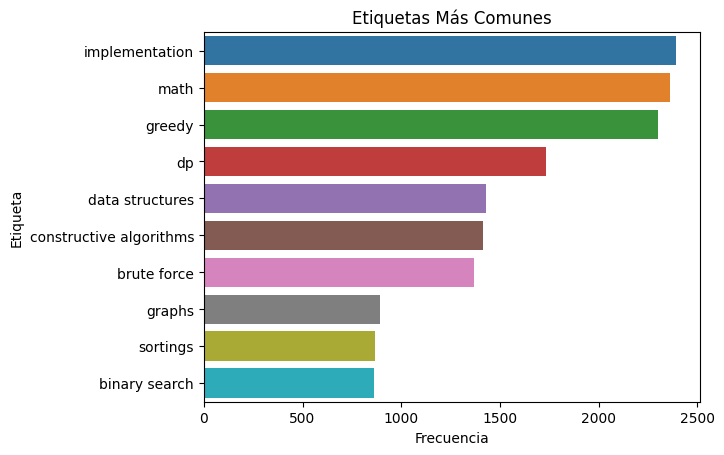
\includegraphics[scale=0.8]{imgs/common_tags_count.png}
          \end{center}
          en la gráfica anterior se puede observar que la etiqueta más común es \textbf{implementation}, esto es bastante común, ya
          que la dificultad de muchos problemas además de la idea radica en la implementación de los algoritmos (sería interesante medir
          como se comporta la clasificación de un problema usando esta etiqueta si solo nos enfocáramos en el código del problema). 
    \item Distribución de idiomas
          \begin{center}
              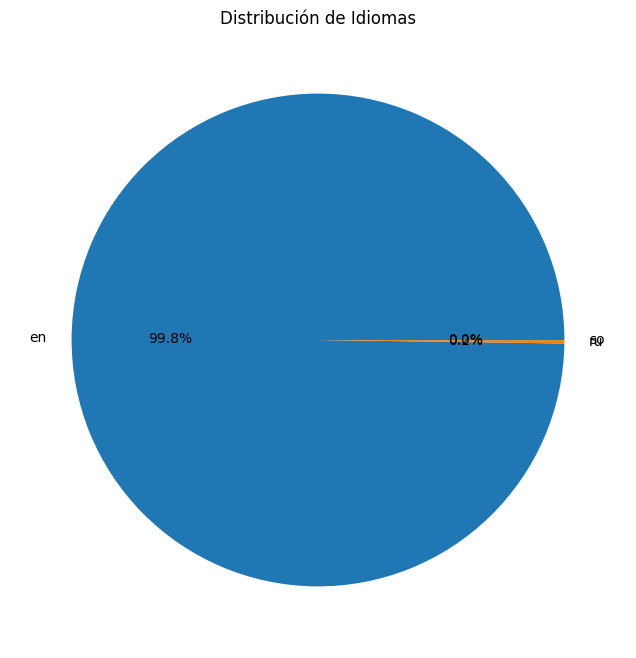
\includegraphics[scale=0.6]{imgs/langs_dist.png}
          \end{center}
          en la gráfica anterior se puede observar que el idioma más común es el \textbf{Inglés} y una pequeña parte en ruso, en este trabajo
          solo consideraremos los ejercicios en idioma \textbf{Inglés}.
          \newpage
          
    \item Nube de palabras asociada a la descripción de los problemas
          \begin{center}
              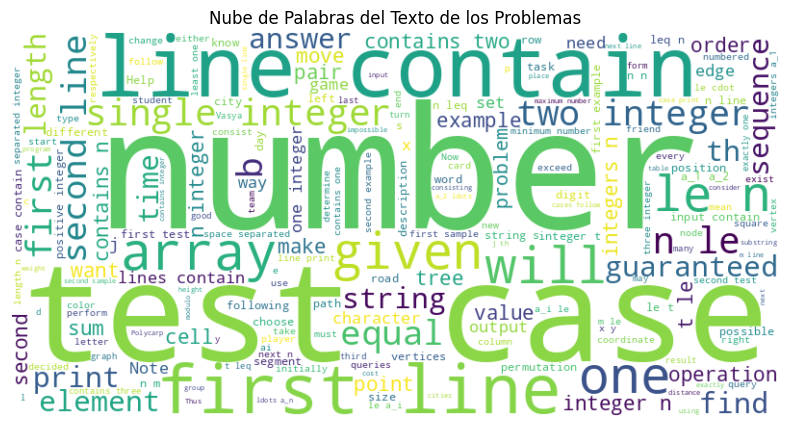
\includegraphics[scale=0.55]{imgs/wordcloud.png}
          \end{center}
          en la gráfica anterior se pueden observar las palabras que más se repiten, la palabra más común es \textbf{Number}, lo que coincide con
          el tema fundamental de estos ejercicio ya que la mayoría tratan problemas relacionados con la Matemática. Después se observan las palabras
          \textbf{test} y \textbf{case}, título de la sección donde se describen los casos de prueba del problema.
          \newpage
          
    \item Matriz de correlación de las etiquetas
          \begin{center}
              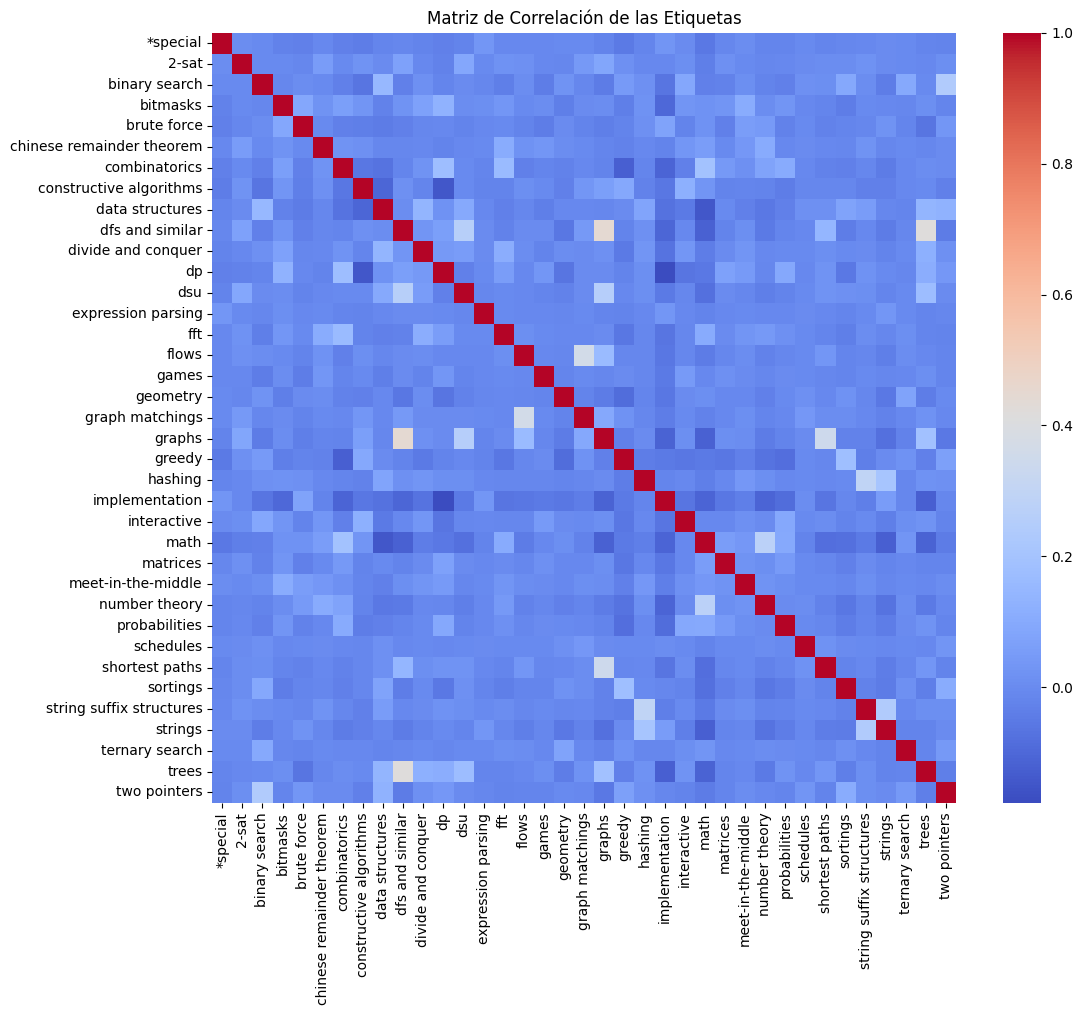
\includegraphics[scale=0.5]{imgs/correlation_matrix.png}
          \end{center}
          en la gráfica anterior se puede observar la matriz de correlación de las etiquetas que muestra para cada para de etiquetas la frecuencia
          de los problemas donde estas se aparecen a la vez. Se puede observar una estrecha relación entre los problemas con las etiquetas \textbf{dfs and similar}, \textbf{graphs} y \textbf{trees}
          (esto tomando cada par de etiquetas donde participan 2 de estas 3, con una mayor relación para el para \textbf{dfs and similar} y \textbf{graphs}), esto a raíz de que para los problemas de grafos
          y en un caso particular de árboles es muy común una vía de solución usando \textbf{DFS}.
          
\end{itemize}

\subsection{Preprocesamiento de datos}

En el preprocesamiento de datos, se realizaron varios pasos para 
limpiar y normalizar los textos de las descripciones y otros campos del 
conjunto de datos. A continuación, se describen las principales etapas 
y funciones utilizadas:

\begin{enumerate}
    \item \textbf{Corrección de capitalización después de puntos}
          \begin{itemize}
              \item \textbf{Función:} \texttt{processing\_dot\_capitalize}
              \item \textbf{Descripción:} Añade un espacio antes de una letra mayúscula si viene después de un punto, para corregir errores de capitalización en los textos.
          \end{itemize}
    \item \textbf{Reemplazo de notación exponencial}
          \begin{itemize}
              \item \textbf{Función:} \texttt{replace\_exponent\_notation}
              \item \textbf{Descripción:} Convierte notaciones como $10^6$ a su equivalente numérico 1000000 usando expresiones regulares.
          \end{itemize}
    \item \textbf{Espaciado entre signos de dólar}
          \begin{itemize}
              \item \textbf{Función:} \texttt{add\_spacing\_between\_dollar\_signs}
              \item \textbf{Descripción:} Añade espacios alrededor de los símbolos \$\$\$ para facilitar el procesamiento posterior.
          \end{itemize}
    \item \textbf{Conversión a minúsculas}
          \begin{itemize}
              \item \textbf{Función:} \texttt{convert\_to\_lowercase}
              \item \textbf{Descripción:} Convierte todo el texto a minúsculas para una normalización uniforme.
          \end{itemize}
    \item \textbf{Cálculo de multiplicaciones en el texto}
          \begin{itemize}
              \item \textbf{Función:} \texttt{calculate\_multiplication}
              \item \textbf{Descripción:} Evalúa y reemplaza expresiones de multiplicación como 2 \textbackslash cdot 100000 por su resultado 200000.
          \end{itemize}
    \item \textbf{Preprocesamiento general}
          \begin{itemize}
              \item \textbf{Función:} \texttt{preprocessing}
              \item \textbf{Descripción:} Aplica todas las funciones anteriores secuencialmente para limpiar y normalizar el texto.
          \end{itemize}
    \item \textbf{Tokenización y lemmatización}
          \begin{itemize}
              \item \textbf{Función:} \texttt{split\_sentences, split\_words, lemmatization}
              \item \textbf{Descripción:} Divide el texto en oraciones y palabras, y aplica lematización para reducir las palabras a su forma base.
          \end{itemize}
    \item \textbf{Eliminación de stopwords}
          \begin{itemize}
              \item \textbf{Función:} \texttt{remove\_stopwords}
              \item \textbf{Descripción:} Elimina palabras comunes (stopwords) para reducir el ruido en los datos.
          \end{itemize}
    \item \textbf{Procesamiento de descripciones}
          \begin{itemize}
              \item \textbf{Función:} \texttt{get\_preprocessed\_sentence}
              \item \textbf{Descripción:} Aplica todas las técnicas de preprocesamiento a cada descripción en el conjunto de datos.
          \end{itemize}
    \item \textbf{Procesamiento de límites de tiempo y memoria}
          \begin{itemize}
              \item \textbf{Descripción:} Convierte los límites de tiempo y memoria a formatos numéricos apropiados, eliminando unidades innecesarias y valores nulos.
          \end{itemize}
    \item \textbf{Eliminación de columnas innecesarias}
          \begin{itemize}
              \item \textbf{Descripción:} Se eliminan columnas no relevantes como \texttt{input\_file} y \texttt{output\_file} para simplificar el conjunto de datos.
          \end{itemize}
\end{enumerate}

En resumen, el preprocesamiento de datos incluyó la normalización y 
limpieza del texto, lematización, eliminación de stopwords, procesamiento 
de signos de dólar, tokenización y el manejo de valores en columnas 
específicas como límites de tiempo y memoria. Estas transformaciones 
aseguraron que los datos estuvieran en un formato adecuado para ser 
utilizados en el modelo de clasificación.


\section{Estado del arte}

\subsection{Revisión bibliográfica}

En la revisión bibliográfica analizado encontramos 2 líneas de investigación fundamentales, modelos que analizaban solo
el lenguaje natural y por otro lado modelos que se enfocaban análisis en el análisis de código (es decir dado el texto o el ast
de un código en un lenguaje específico daba como salida los tags asociados a dicho código). A continuación se relacionan los 
papers estudiados.

\begin{itemize}
    \item Preprocesamiento de Lenguaje Natural
          
          \begin{longtable}{|p{2cm}|p{0.8cm}|p{2cm}|p{2cm}|p{3cm}|p{2cm}|p{3cm}|}
              \hline
              \textbf{Paper} & \textbf{Año}                                                                                                                                                       & \textbf{Link} & \textbf{Modelos} & \textbf{Resultados} & \textbf{Dataset} & \textbf{Métodos} \\
              \hline
              \endfirsthead
              
              \hline
              \endfoot
              
              \hline
              \endlastfoot
              
              
              Predicting algorithmic approach for programming problems from natural language problem description 
                             & 2016 
                             & \href{https://ashishbora.github.io/assets/projects/nlp/report.pdf}{\url{https://ashishbora.github.io/assets/projects/nlp/report.pdf}}

              
              
              
              
              
                             & Long Short Term Memory (LSTM), Random Forest, clasificador dummy
                             & Solamente Random Forest presentó mejoras sobre el clasificador dummy, el cual predijo el tag más común
                             & Codeforces, considerando solo el primer tag para cada problema
                             & Vectores word2vec pre entrenado y codificación one-hot para representar la entrada de datos                                                                                                                                                                             \\
              
              \hline
              Predicting algorithm classes for programming word problems
                             & 2019
                             & \href{https://aclanthology.org/D19-5511/}{\url{https://aclanthology.org/D19-5511/}}

              
              
              
              
              
                             & Convolutional Neural Networks (CNN), ensemble de CNNs, predicciones humanas
                             & Mejores resultados para el ensemble de CNNs; las predicciones humanas tuvieron mejores resultados que el resto de los modelos pero con una puntuación de 0.43 del macro-F1 en la clasificación multietiqueta de los primeros 20 
                             & Codeforces, prediciendo 10 y 20 de los tags más frequentes
                             & Acercamientos de clasificación mulitclase y multietiqueta para la predicción de los tags                                                                                                                                                                       \\
              
              \hline
              Multi-label classification for automatic tag prediction in the context of programming challenges
                             & 2019
                             & \href{https://arxiv.org/abs/1911.12224}{\url{https://arxiv.org/abs/1911.12224}}

              
              
              
              
              
              
                             & Long Short Term Memory (LSTM)
                             & Mejor puntuación F1 para LSTM sobre la codificación one-hot; mejor Weighted Hamming Score para LSTM sobre word2vec
                             & Codeforces y TopCoder, tags ordenados en 9 clases
                             & Doc2Vec, LSTM sobre word2vec, LSTM sobre codificación one-hot                                                                                                                                                                                                \\
              
              \hline
              Classification of Programming Problems based on Topic Modeling
                             & 2019
                             & \href{https://dl.acm.org/doi/10.1145/3323771.3323795}{\url{https://dl.acm.org/doi/10.1145/3323771.3323795}}

              
              
              
              
              
              
                             & k-Nearest Neighbors (kNN), Random Forest (RF), Multinomial Naive Bayes (MNB), Multilayer Perceptron (MLP) 
                             & La precisión final no mejoró mucho en comparación con la línea de base de TF-IDF (0,86 frente a 0,88 de precisión); impacto positivo en kNN y MNB, negativo en RF 
                             & 
                             & Modelado de temas (LDA, NMF) para vectorización; algoritmos de clasificación: kNN, RF, MNB, MLP                                                                                                                                                                      \\
              
              \hline
              
          \end{longtable}
          
    \item Análisis de Código
          
          \begin{longtable}{|p{2cm}|p{0.8cm}|p{2cm}|p{2cm}|p{3cm}|p{2cm}|p{3cm}|}
              \hline
              \textbf{Paper} & \textbf{Año}                                                                                                                                                                                                                                                                                               & \textbf{Link} & \textbf{Modelos} & \textbf{Resultados} & \textbf{Dataset} & \textbf{Métodos} \\
              \hline
              \endfirsthead
              
              \hline
              \endfoot
              
              \hline
              \endlastfoot
              
              
              Automatic algorithm recognition of source-code using machine
              learning
                             & 2017
                             & \href{https://www.semanticscholar.org/paper/Automatic_Algorithm_Recognition_of_Source_Code_Shalaby_Mehrez/641beb8d201a9bda_27dd0b5a7727116_cd47c7cb9}{\url{https://www.semanticscholar.org/paper/Automatic_Algorithm_Recognition_of_Source_Code_Shalaby_Mehrez/641beb8d201a9bda_27dd0b5a7727116_cd47c7cb9}}

              
              
              
              
              
                             & Algoritmos de clasificación tradicionales
                             & Aplicación exitosa de algoritmos de clasificación tradicionales y métricas de código para clasificar soluciones
                             & Codeforces 
                             & Enfoque basado en métricas para la vectorización del código fuente; 30 métricas de software diferentes (por ejemplo, número de variables de tipos específicos, líneas de código, número de bucles, número de bucles anidados)                                                                                                                                                                                                                \\
              
              \hline
              Classification and recommendation of competitive programming problems
              using CNN
                             & 2017
                             & \href{https://www.researchgate.net/publication/321868484_Classification_and_Recommendation_of_Competitive_Programming_Problems_Using_CNN}{\url{https://www.researchgate.net/publication/321868484_Classification_and_Recommendation_of_Competitive_Programming_Problems_Using_CNN}}

              
              
              
              
              
                             & CNN a nivel de caracteres
                             & Logró clasificar las soluciones en cuatro clases; Combinación de información de todas las soluciones presentadas: clasificación mejorada 
                             & Codeforces 
                             & CNN a nivel de caracteres; propuso combinar la información de las clasificaciones de las soluciones individuales                                                                                                                                                                                                                                                                                                       \\
              
              \hline
              
          \end{longtable}
          
          
\end{itemize}

\section{Propuestas de solución}
\subsection{Clasificación Multietiqueta con TF-IDF y Naive Bayes}
La clasificación multietiqueta es una variante de la clasificación en la que cada instancia puede pertenecer a múltiples clases simultáneamente. En este estudio, utilizamos la vectorización TF-IDF para la extracción de características y un clasificador Naive Bayes para la clasificación. El objetivo principal es evaluar el rendimiento del modelo en varias métricas de evaluación.
\subsection{Clasificación Multietiqueta con TF-IDF y KNN}
Al igual que en la sección anterior, usaremos el enfoque de modelo de aprendizaje multietiquetas. La vectorización usada es la misma que en Naive-Bayes, TF-IDF para extraer características y un clasificador KNN para la clasificación. El objetivo poder comparar el rendimiento de este modelo con los otros que hemos usado.

\subsection{Clasificación Multietiqueta usando Deep Learning}

Durante el estudio del estado del arte notamos que un clasificador de algoritmos dado el texto 
basado en CNN puede lograr un rendimiento casi humano. Sin embargo, estas las arquitecturas 
presentadas no manejan eficazmente secuencias largas, que son comunes en las descripciones de 
problemas de esta índole. Para abordar esta limitación, adoptamos arquitecturas recientes 
basadas en transformers, que son más adecuadas para manejar secuencias largas. Nuestro método 
aborda la clasificación de etiquetas múltiples, ya que cada problema de algoritmo puede 
pertenecer a varias etiquetas simultáneamente.

Para lograr esto se define una función $F$ como un extractor de features que convierte un 
texto en un espacio de representaciones vectoriales (embeddings). Luego, utilizamos una cabeza 
de clasificación $H$ sobre el extractor. Nuestro modelo resuelve el problema de la 
clasificación de etiquetas múltiples usando una función de pérdida de entropía cruzada binaria:

$$
    E_{(x, y) \in D_{train}} [ l(H(F(x)), y) ]
$$

donde $l$ es una pérdida de entropía cruzada binaria para las categorías $y$ del problema $x$.

Recolectamos en total 7968 problemas de algoritmos de CodeForces, con 37 etiquetas distintas. 
Utilizamos un extractor de features basado en BERT y una red de cabeza de 
clasificación. Usamos la arquitectura \href{https://huggingface.co/google/bigbird-roberta-base}{BigBird}
en nuestra modelación que nos permite introducir extensas secuencias de tokens.

\section{Experimentación y resultados}

\subsection{Clasificación Multietiqueta con TF-IDF y Naive Bayes}
\subsubsection{Metodología}
\begin{itemize}
    \item Preprocesamiento de Datos
\end{itemize}
El conjunto de datos preprocesado pasa a utilizar la vectorización TF-IDF para convertir los datos de texto en características numéricas. Las etiquetas se transformaron a un vector binario utilizando \texttt{MultiLabelBinarizer} para adaptarse a la naturaleza multietiqueta del problema.

\begin{itemize}
    \item Entrenamiento del Modelo
\end{itemize}
La clasificación se realizó utilizando un clasificador Naive Bayes dentro de un marco One-vs-Rest. El conjunto de datos se dividió en conjuntos de entrenamiento y prueba utilizando una división 80-20. Una vez el modelo predecía habían problemas a los cuales no se les
asignaba ninguna etiqueta, cosa que no sucede en el codeforces, por lo cual se le hace asignar a dichos problemas la etiqueta más probable, garantizando así que todo problema contenga al menos una etiqueta.

\begin{lstlisting}[language=Python, caption=Naive Bayes]
vectorizer = TfidfVectorizer()
X = vectorizer.fit_transform(text_data)
mlb = MultiLabelBinarizer()
y = mlb.fit_transform(labels)

X_train, X_test, y_train, y_test = train_test_split(X, y, test_size=0.2, random_state=42)

clf = OneVsRestClassifier(MultinomialNB())
clf.fit(X_train, y_train)
y_pred = clf.predict(X_test)
\end{lstlisting}
\newpage

\subsubsection{Resultados}
\begin{table}[ht!]
    \centering
    \begin{minipage}{0.45\textwidth}
        \centering
        \begin{tabular}{lr}
            \toprule
            {}                      & auc-roc  \\
            \midrule
            brute force             & 0.50440  \\
            constructive algorithms & 0.50000  \\
            data structures         & 0.51020  \\
            dfs and similar         & 0.50000  \\
            dp                      & 0.50000  \\
            geometry                & 0.52941  \\
            greedy                  & 0.59057  \\
            implementation          & 0.62189  \\
            math                    & 0.52669  \\
            strings                 & 0.62795  \\
            \bottomrule
        \end{tabular}
        \caption{ROC-AUC Scores}
    \end{minipage}%
    \hspace{0.05\textwidth} % Espacio entre tablas
    \begin{minipage}{0.45\textwidth}
        \centering
        \begin{tabular}{lr}
            \toprule
            {}                      & auc-roc  \\
            \midrule
            brute force             & 0.50062  \\
            constructive algorithms & 0.50486  \\
            data structures         & 0.52040  \\
            dfs and similar         & 0.50000  \\
            dp                      & 0.50000  \\
            geometry                & 0.58823  \\
            greedy                  & 0.60907  \\
            implementation          & 0.59370  \\
            math                    & 0.60561  \\
            strings                 & 0.68182  \\
            \bottomrule
        \end{tabular}
        \caption{ROC-AUC Scores (Al menos una etiqueta por problema)}
    \end{minipage}
\end{table}
\newpage

\begin{itemize}
    \item F1 Score:
\end{itemize}
\begin{verbatim}
F1 Score: 0.16300
F1 Score (Al menos un tag por problema): 0.23954
\end{verbatim}
\begin{itemize}
    \item ROC-AUC Score:
\end{itemize}
\begin{verbatim}
ROC-AUC Score: 0.54111
ROC-AUC Score (Al menos un tag por problema): 0.56043
\end{verbatim}
\begin{itemize}
    \item Umbral de Decisi\'on usado (Ambos Casos):
\end{itemize}
\begin{verbatim}
Umbral de Decisión: 0.5
\end{verbatim}
\begin{figure}[H]
    \centering
    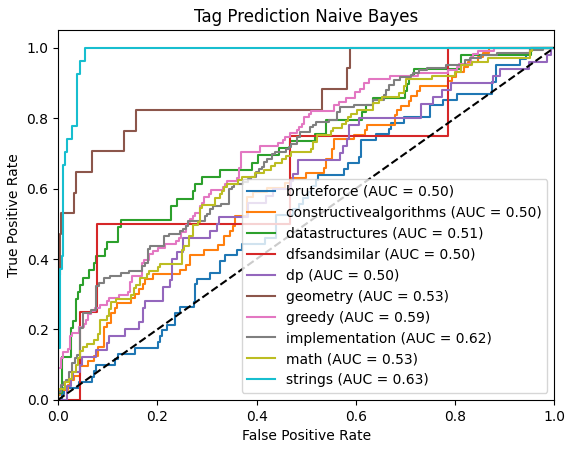
\includegraphics[scale=0.7]{imgs/roc_auc_nb.png}
    \caption{Tags ROC-AUC}
    \label{fig:ranb}
\end{figure}
Como se pude apreciar el agregarle la etiqueta más probable a aquellos problemas que no les fueron asignados por el modelo ninguna etiqueta hace una mejora en los resultados obtenidos en casi todas las métricas usadas, solo las etiqueta brute force  e implementation obtienen un mejor valor en roc-auc sin hacer esto, lo cual está dado a que aquellos problemas sin etiquetar se le haya asignado su etiqueta incorrectamente .\\\newline

\newpage

\subsection{Clasificación Multietiqueta con TF-IDF y KNN}
\subsubsection{Metodología}
\begin{itemize}
    \item Preprocesamiento de Datos
\end{itemize}
además de preprocesar la descripción de los problemas para usar TF-IDF, al ser KNN un modelo que solo se puede entrenar con valores numéricos, también se binarizaron los tags de los problemas, y se eliminaron columnas poco relevantes como el idioma y la identificación de los problemas.

\begin{itemize}
    \item Entrenamiento del Modelo
\end{itemize}
La clasificación se realizó utilizando un clasificador KNN dentro de un marco MultiOutput. El conjunto de datos se dividió en conjuntos de entrenamiento y prueba utilizando una división 80-20.\\ 
Pero cuál sería el mejor valor de K para el modelo, para esto se realizó una búsqueda de hiperparámetros con valores de K de 1 a 100, dando como resultado que K = 12 era el valor con mayor precisión en los resultados.

\begin{lstlisting}[language=Python, caption=KNN]
    
    X_train, X_test, y_train, y_test = train_test_split(X, y, test_size=0.2, random_state=42)
    
    neighbors = np.arange(1, 100)
    train_accuracies = {}
    test_accuracies = {}
    reports = []
    for neighbor in neighbors:
        knn = KNeighborsClassifier(n_neighbors=neighbor)
        mlb_knn = MultiOutputClassifier(knn)
        mlb_knn.fit(X_train, y_train)
        ypred = mlb_knn.predict(X_test) 
        train_accuracies[neighbor] = mlb_knn.score(X_train, y_train)
        test_accuracies[neighbor] = mlb_knn.score(X_test, y_test)
        reports.append(classification_report(y_test, ypred, zero_division = 0))
    \end{lstlisting}

\subsubsection{Resultados}
\begin{itemize}
    \item Informe de Clasificación
\end{itemize}

\begin{verbatim}
report = classification_report(y_test, y_pred, target_names=list(all_tags))
\end{verbatim}

\begin{tabular}{lrrrr}
    \toprule
                           & precision & recall   & f1-score & support    \\
    \midrule
    math                   & 0.410256  & 0.163265 & 0.233577 & 98.000000  \\
    strings                & 0.555556  & 0.500000 & 0.526316 & 30.000000  \\
    datastructures         & 0.900000  & 0.209302 & 0.339623 & 43.000000  \\
    greedy                 & 0.500000  & 0.350000 & 0.411765 & 100.000000 \\
    dfsandsimilar          & 0.000000  & 0.000000 & 0.000000 & 10.000000  \\
    constructivealgorithms & 0.100000  & 0.017544 & 0.029851 & 57.000000  \\
    implementation         & 0.602740  & 0.325926 & 0.423077 & 135.000000 \\
    geometry               & 1.000000  & 0.062500 & 0.117647 & 16.000000  \\
    bruteforce             & 0.500000  & 0.015152 & 0.029412 & 66.000000  \\
    dp                     & 0.000000  & 0.000000 & 0.000000 & 47.000000  \\
    \bottomrule
\end{tabular}

\begin{itemize}
    \item Accuracy
\end{itemize}
\begin{verbatim}
Overall Accuracy: 8.00\%
\end{verbatim}

\newpage
\begin{itemize}
    \item Precision ,F1-Score ,Recall y Support para cada etiqueta
\end{itemize}
\begin{figure}[H]
    \centering
    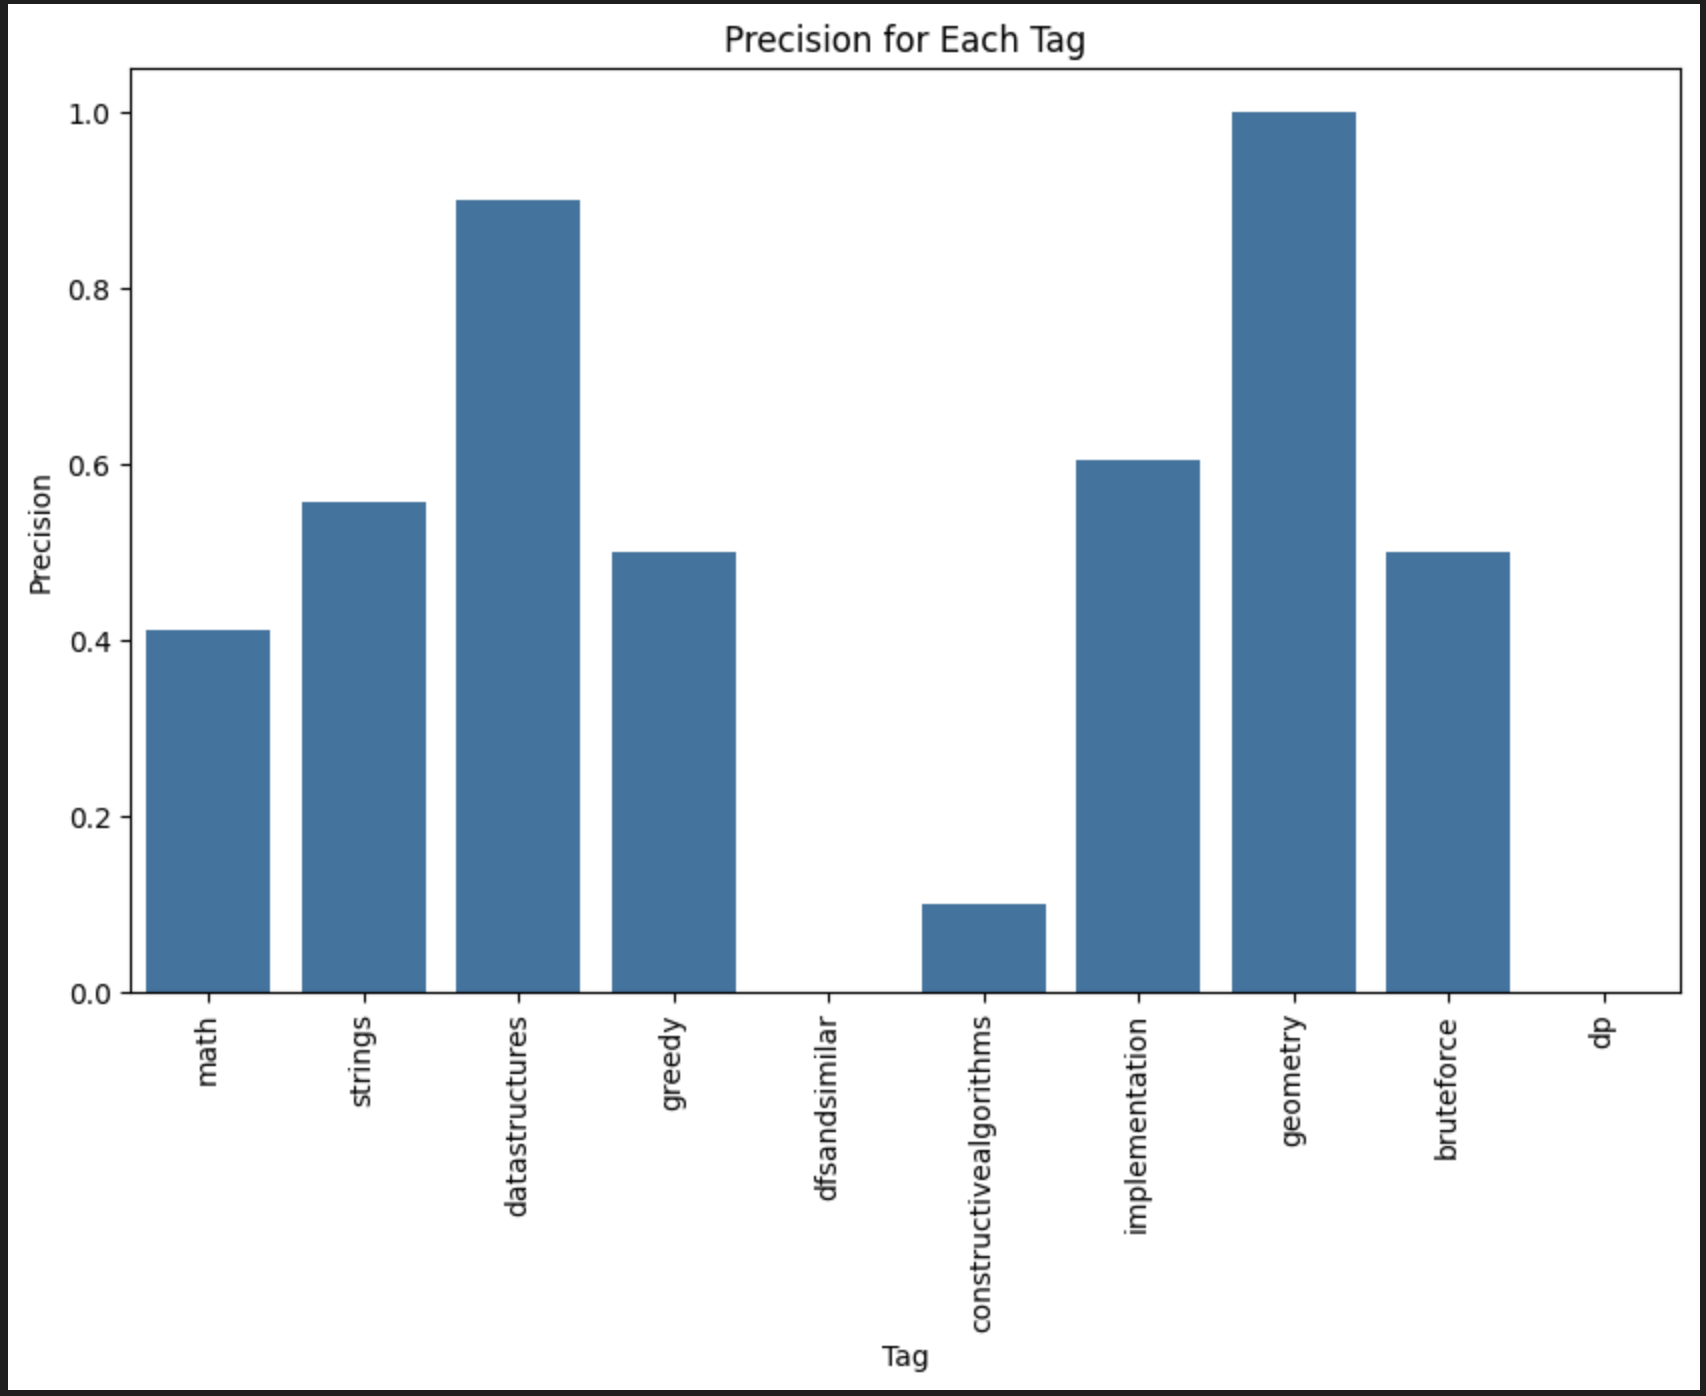
\includegraphics[scale=0.49]{imgs/precisonknn.png}
    \caption{Precision}
    \label{fig:p}
\end{figure}
\begin{figure}[H]
    \centering
    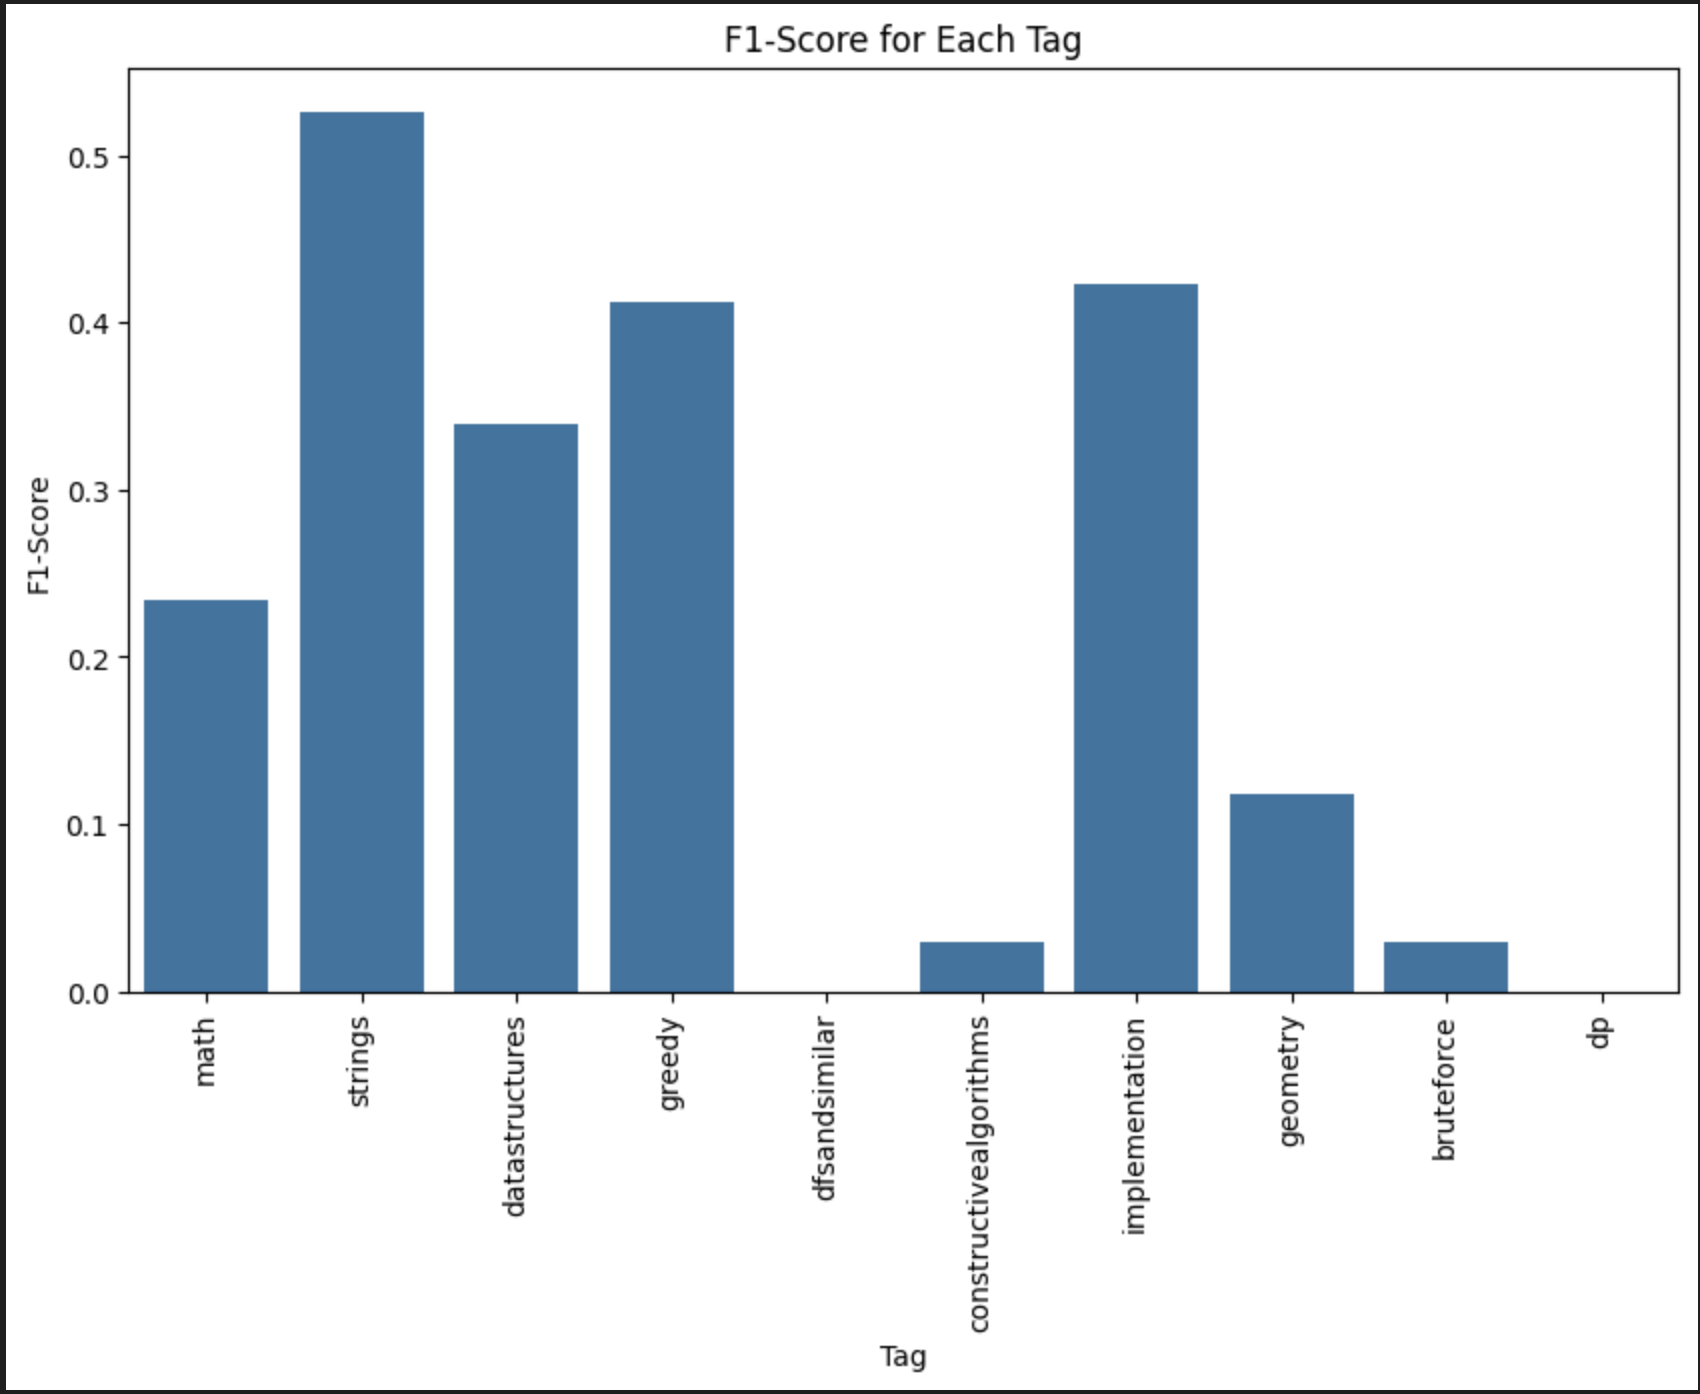
\includegraphics[scale=0.49]{imgs/f1knn.png}
    \caption{F1-Score}
    \label{fig:f1}
\end{figure}
\begin{figure}[H]
    \centering
    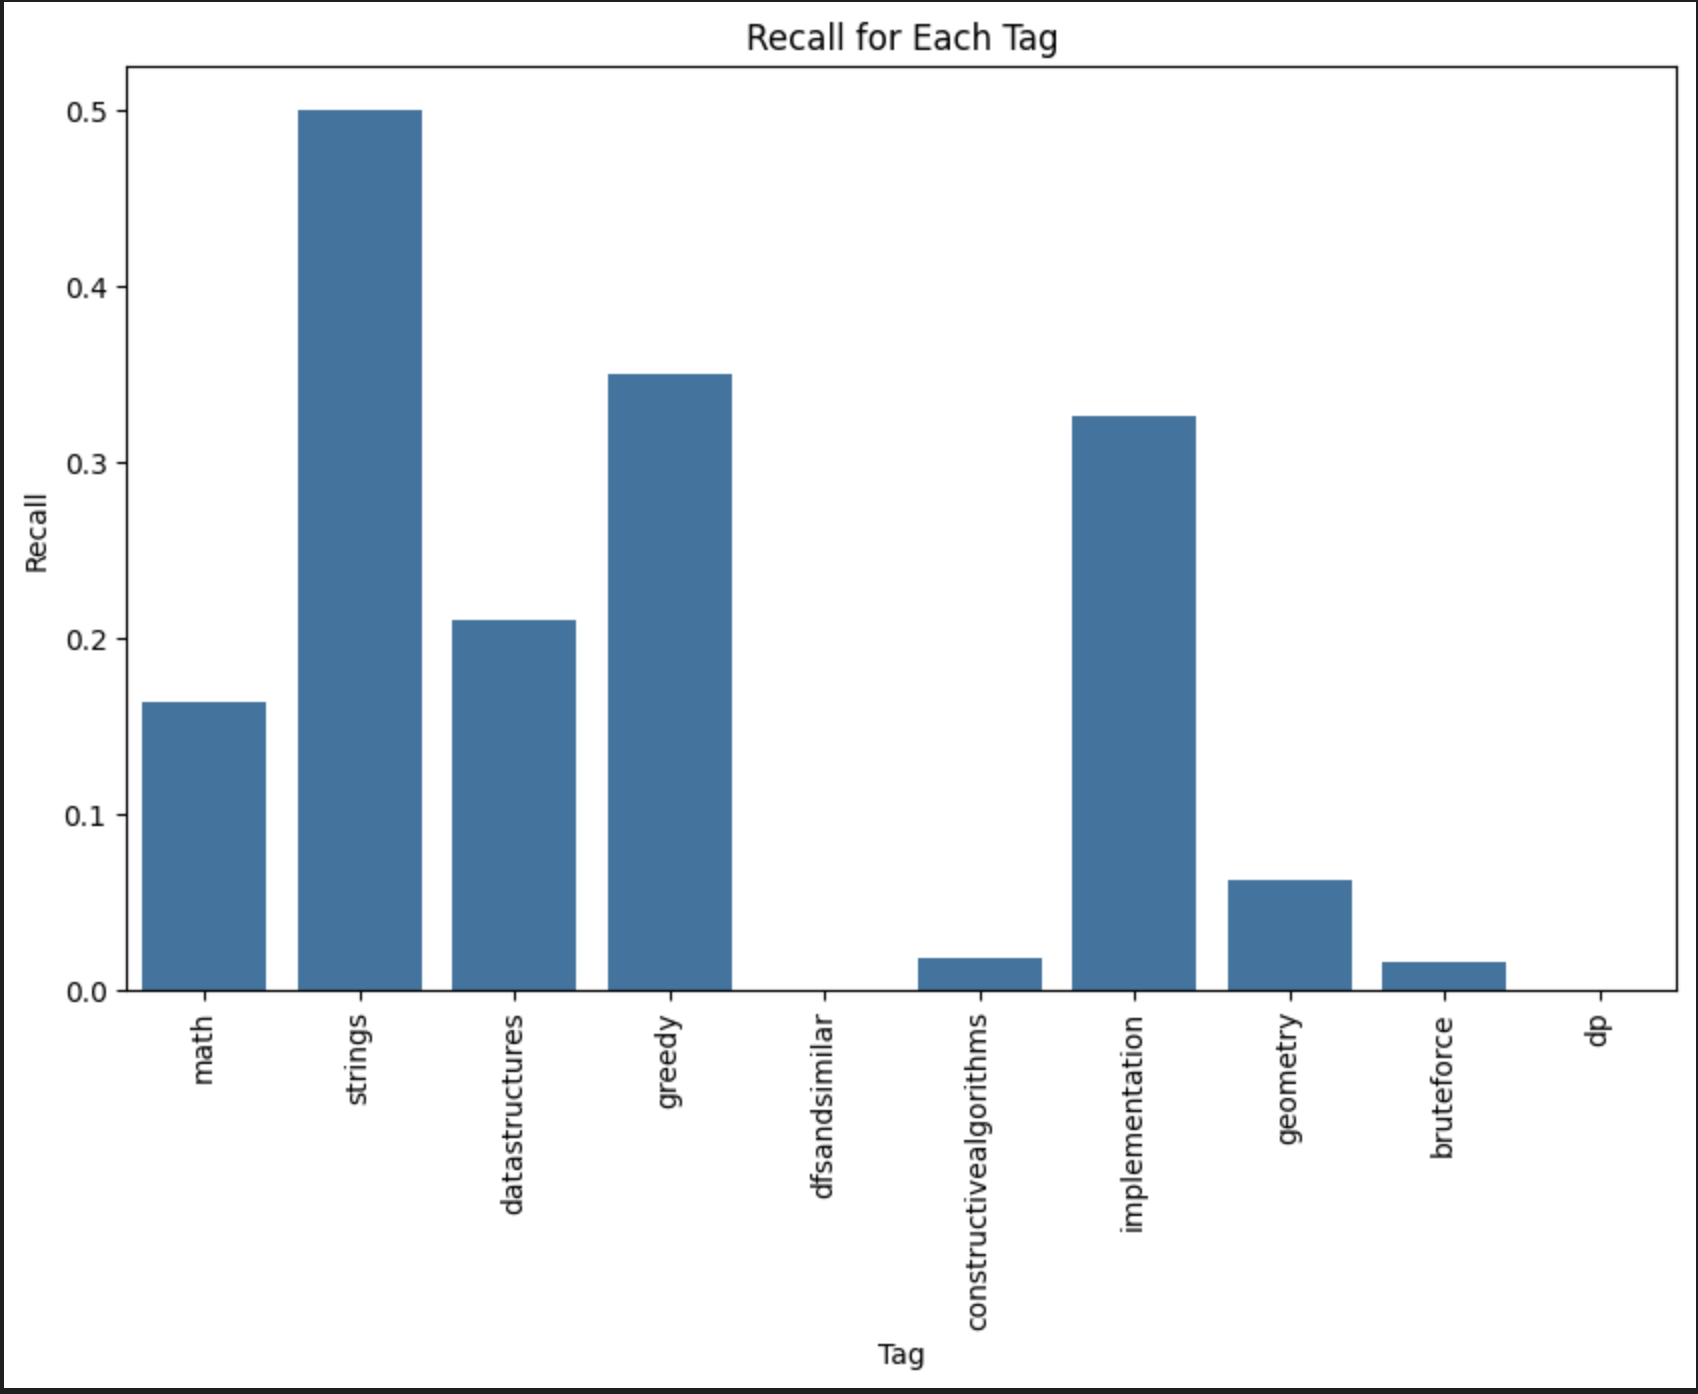
\includegraphics[scale=0.49]{imgs/recallknn.png}
    \caption{Recall}
    \label{fig:r}
\end{figure}
\begin{figure}[H]
    \centering
    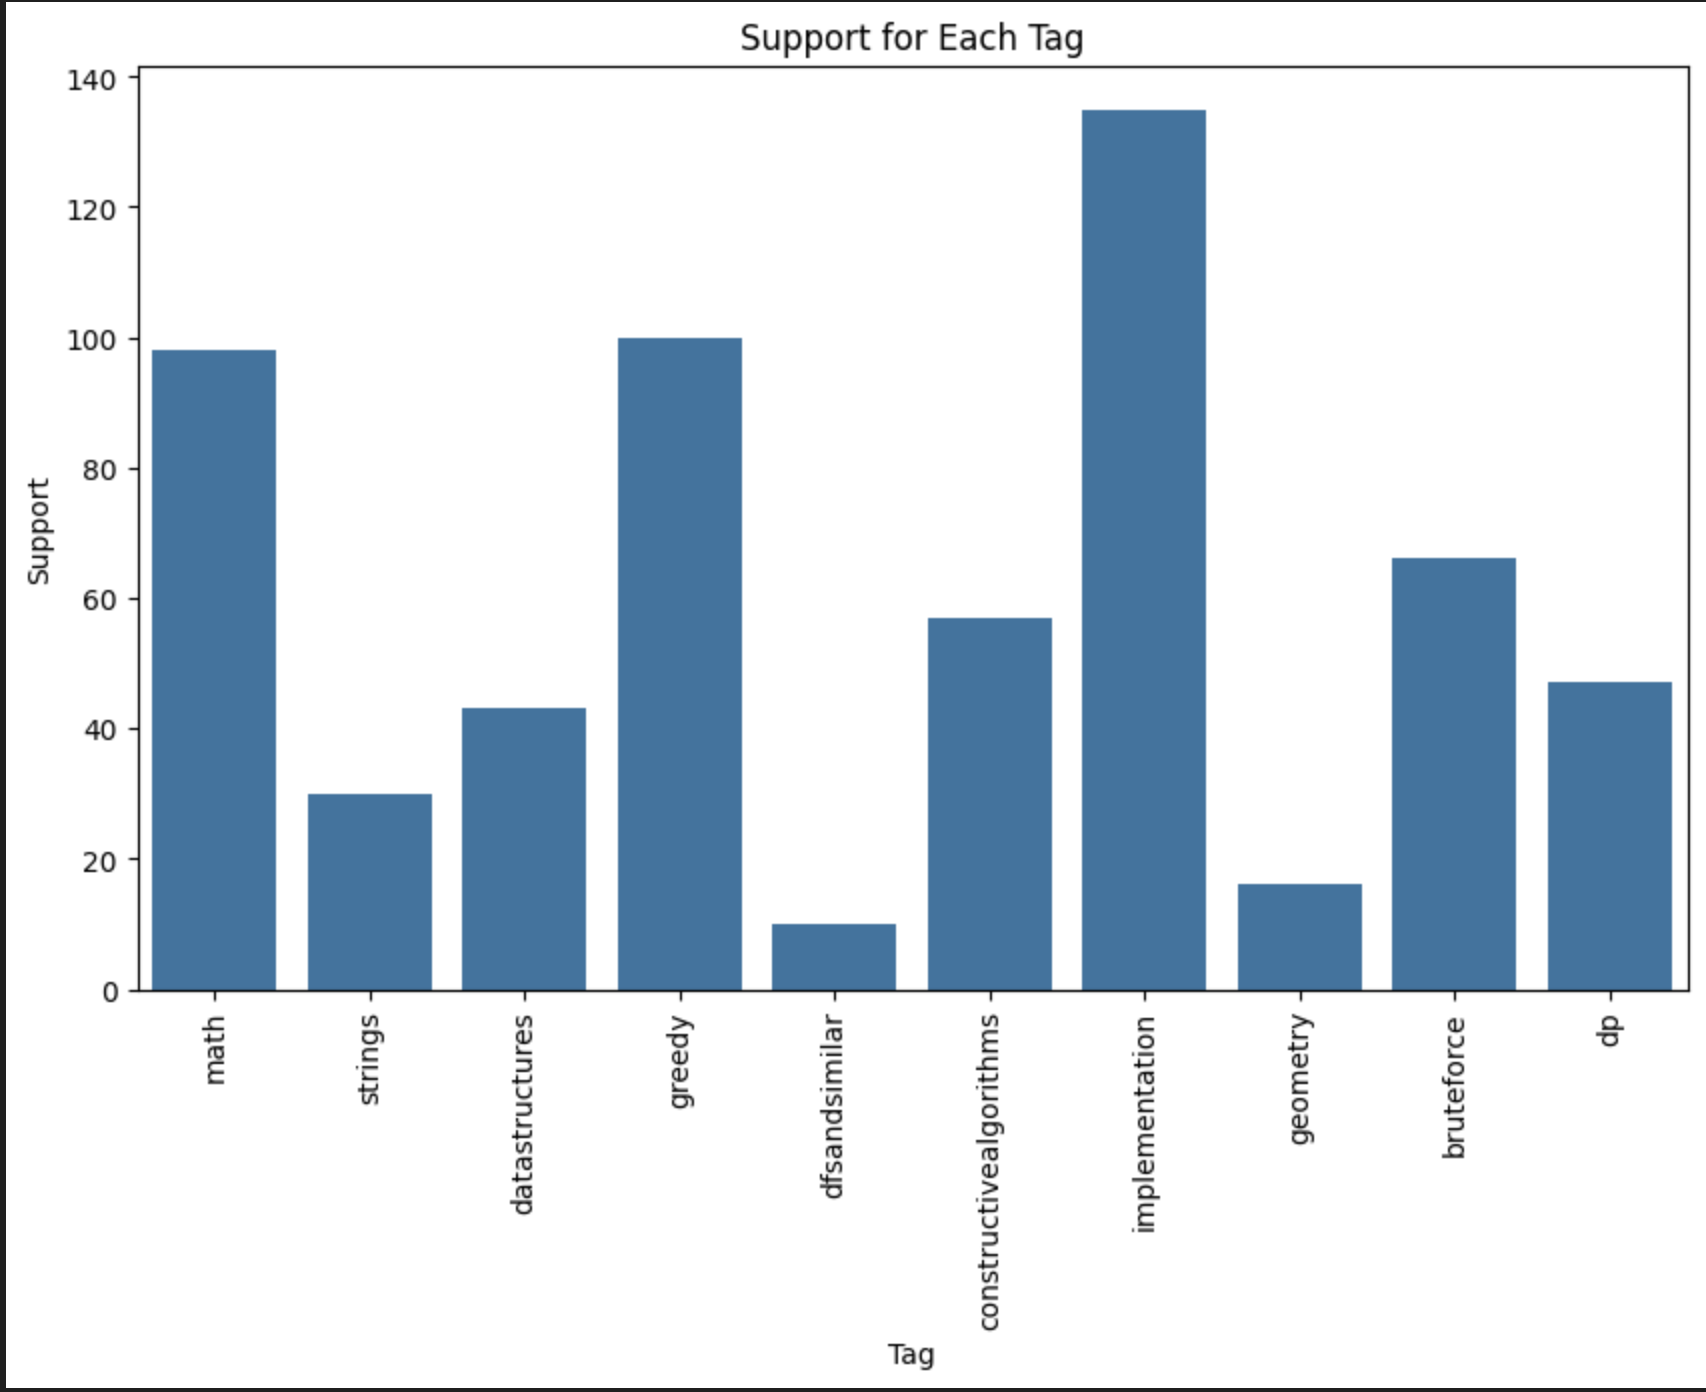
\includegraphics[scale=0.49]{imgs/supportkn.png}
    \caption{Support}
    \label{fig:s}
\end{figure}

\subsection{Clasificación Multietiqueta usando Deep Learning}

A pesar de haber recolectado un dataset de problemas tan extenso, por cuestiones de 
rapidez en el cómputo decidimos solo usar 1625 de ellos, la mitad 
del total teniendo en cuenta únicamente los problemas que solo están 
tagueados con las etiquetas más comunes. En nuestros experimentos, evaluamos varias configuraciones 
iniciales para el entrenamiento del modelo de clasificación de texto con el objetivo de 
validar la efectividad de nuestro conjunto de datos propuesto. Sin embargo, no nos fue posible 
concluirlo, pudiendo completar solo el 25\% de las epochs previstas. Estos fueron los resultados 
alcanzados en el último checkpoint de nuestro modelo:

\begin{tabular}{lrrrr}
    \toprule
    {}                      & auc-roc \\
    \midrule
    brute force             & 0.53433 \\
    constructiv ealgorithms & 0.60461 \\
    data structures         & 0.55745 \\
    dfs and similar         & 0.39719 \\
    dp                      & 0.53294 \\
    geometry                & 0.64132 \\
    greedy                  & 0.62073 \\
    implementation          & 0.60420 \\
    math                    & 0.65266 \\
    strings                 & 0.67921 \\
    \bottomrule
\end{tabular}

\begin{itemize}
    \item \textbf{ROC-AUC Score = $0.5824715558064865$}: Esta métrica indica que, en promedio, el modelo tiene una
          capacidad moderada para distinguir entre las clases. Un valor de 0.5 sugiere que el modelo 
          no tiene mejor rendimiento que una clasificación aleatoria, mientras que un valor de 1 
          indica una clasificación perfecta. Por lo tanto, un AUC-ROC de aproximadamente 0.582 sugiere 
          que hay margen para mejorar el modelo. AUC-ROC  es el Área Bajo la Curva del Receptor Operador 
          Característico.
    \item \textbf{F1 Score = $0.3080225264908538$}: El F1 score combina precisión y recall en una
          sola métrica. Un valor de 0.308 indica que el modelo tiene un rendimiento bajo en términos de 
          equilibrio entre estos dos aspectos. Nuevamente, esto sugiere que hay espacio para mejoras.
    \item \textbf{Umbral de decisión = $0.001$}: Este valor indica el umbral utilizado para convertir las
          probabilidades de las etiquetas en predicciones binarias. Un umbral tan bajo podría estar 
          indicando que el modelo está tratando de ser muy inclusivo (es decir, prefiere clasificar 
          algo como positivo con una probabilidad muy baja), lo cual evidentemente está afectando la 
          precisión de las predicciones.
\end{itemize}

\begin{figure}[H]
    \centering
    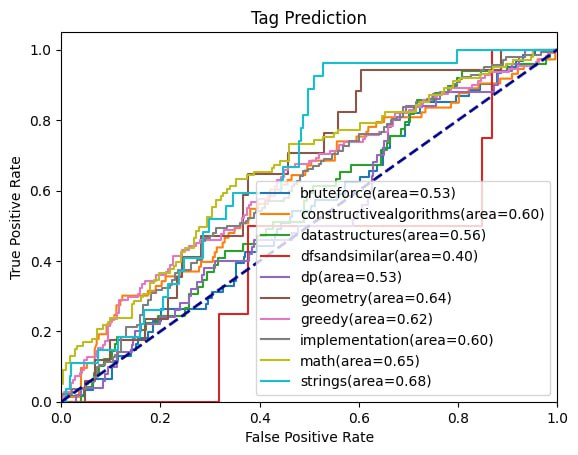
\includegraphics[scale=0.55]{imgs/roc_auc.jpg}
    \caption{Tags ROC-AUC}
\end{figure}

Dado el rendimiento moderado en AUC-ROC y bajo en F1 score, además de la variabilidad notable en 
el rendimiento del modelo entre diferentes etiquetas se podría explorar mejorar el 
preprocesamiento de datos, el ajuste de hiperparámetros del modelo, o incluso el uso de técnicas 
de balanceo de clases para obtener mejores métricas.


\subsection{Chat GPT}

Para analizar que tan bien se comportaba Chat GPT 3.5, prediciendo los tags de Codeforces, usamos prompt engineering
con un preprocesamiento sobre los problemas:

\begin{lstlisting}[language=Python, caption=Prompt para tagear los problemas]
def prompt(description):
    all_tags_str = ', '.join(all_tags)
    return f'Give this set of {all_tags_str} tags and this problem ${description}, give me the set of problem tags in the following format: greedy, implementation, dp'
\end{lstlisting}

\begin{tabular}{|l|l|r|r|r|r|}
    \toprule
    {} & Metric        & ChatGPT  & Naive Bayes & KNN      & Deep Learning       \\
    \midrule
    0  & Accuracy      & 0.020000 & 0.146000    & 0.080000 & 0.12615384615384614 \\
    1  & F1 (macro)    & 0.002431 & 0.240000    & 0.210000 & 0.3012989902488488  \\
    2  & F1 (micro)    & 0.020000 & 0.390000    & 0.290000 & 0.4228110599078341  \\
    3  & F1 (weighted) & 0.017556 & 0.320000    & 0.260000 & 0.3973457965486768  \\
    4  & F1 (samples)  & 0.002431 & 0.390000    & 0.240000 & 0.4023785103785104  \\
    \bottomrule
\end{tabular}

En el resto de los modelos comparados se obtuvieron mejores métricas en general, también vale destacar que no nos fue posible
usar ChatGPT 4o, modelo de mayor complejidad con le que esperamos que se comporte mejor, además de que solo nos fue posible 
analizar con ChatGPT 100 problemas ya que no disponíamos de la api y todo el trabajo se realizo de manera manual. Otro aspecto
a destacar, fue que en la mayoría de los problemas ChatGPT respondió  con los tags que se le mostraban de ejemplo en el prompt
lo que en alguna medida demuestra que el modelo en alguno o la mayoría de los casos alucinaba, algo que es común en estos modelos 
de lenguaje.

\section{Discusión de los resultados}
Los resultados obtenidos muestran una clara variabilidad en el rendimiento de los modelos utilizados para la tarea de etiquetado de problemas de Codeforces. A continuación se discuten las observaciones clave de las métricas presentadas:

\begin{itemize}
    \item \textbf{Accuracy:} El modelo basado en ChatGPT presentó la menor precisión (0.020000), indicando que el modelo no fue efectivo en predecir las etiquetas correctas de los problemas. Por otro lado, el modelo de Deep Learning alcanzó la mayor precisión (0.12615384615384614), seguido por Naive Bayes (0.146000). Aunque estas precisiones son bajas, el modelo de Deep Learning muestra un rendimiento relativamente mejor.
          
    \item \textbf{F1 (macro):} Esta métrica mide el equilibrio entre la precisión y el recall para cada clase y promedia estos valores. Aquí, el modelo de Deep Learning obtuvo el valor más alto (0.3012989902488488), indicando un mejor desempeño general en todas las etiquetas. Naive Bayes y KNN también mostraron un rendimiento aceptable con valores de 0.240000 y 0.210000 respectivamente.
          
    \item \textbf{F1 (micro):} El F1 (micro) considera el total de verdaderos positivos, falsos negativos y falsos positivos. Los modelos Naive Bayes y Deep Learning destacaron con valores de 0.390000 y 0.4228110599078341 respectivamente. Estos resultados sugieren que, en términos de equilibrio global, ambos modelos gestionan bien la clasificación de las etiquetas.
          
    \item \textbf{F1 (weighted):} Similar al F1 (macro), pero ponderado por el soporte (número de verdaderos ejemplos en cada clase). Deep Learning nuevamente mostró el mejor desempeño (0.3973457965486768), seguido por Naive Bayes (0.320000). Este resultado indica que el modelo de Deep Learning maneja mejor las clases con un mayor número de ejemplos.
          
    \item \textbf{F1 (samples):} Esta métrica evalúa el rendimiento medio de la clasificación de etiquetas para cada muestra. El modelo de Deep Learning logró el mayor valor (0.4023785103785104), destacando su capacidad para predecir múltiples etiquetas por problema con mayor precisión. Naive Bayes también obtuvo un valor alto (0.390000), indicando un buen rendimiento en esta métrica.
          
\end{itemize}

En resumen, aunque ninguno de los modelos alcanzó un rendimiento excelente, el modelo de Deep Learning mostró un rendimiento superior en la mayoría de las métricas, seguido por Naive Bayes. Estos resultados sugieren que, con ajustes y mejoras adicionales, el enfoque de Deep Learning podría ser más efectivo para la tarea de etiquetado de problemas de Codeforces.

También debemos señalar que como repercusión ética este trabajo puede ser maliciosamente utilizado en concursos online de 
programación competitiva, donde se tiene tolerancia cero al fraude tagueando los problemas 
y de esta manera saber con que idea atacar, aunque cabe destacar que los problemas usualmente no son tan triviales. También positivamente este trabajo es una excelente forma de que en la preparación individual en vista a competencias se pueda utilizar para solo concentrarse en problemas que tengan una etiqueta específica, además creemos que los modelos están abiertos a problemas no solo del propio codeforce, sino de otras plataformas de programación competitiva. Las ideas abordadas en el trabajo
estarán en disposición de todo aquel que quiera seguir avanzando con el tema en cuestión.

\section{Conclusiones}

En este proyecto, nos propusimos desarrollar un sistema de etiquetado automático para problemas de programación competitiva en la plataforma Codeforces utilizando técnicas de \textit{machine learning}. Para ello, empleamos diversos modelos, incluyendo \textit{k-Nearest Neighbors} (k-NN), Naive Bayes, ChatGPT 3.5 y un modelo basado en \textit{embeddings} de texto usando Transformers. A lo largo del desarrollo, enfrentamos varios desafíos, entre ellos la naturaleza multi-etiqueta del problema y la diversidad de los enunciados de los problemas.

Nuestros resultados indican que, si bien los modelos implementados lograron etiquetar algunos problemas correctamente y los resultados son bastante superiores a los arrojados por ChatGPT 3.5, el rendimiento general no fue tan bueno como esperábamos. Las métricas de precisión, \textit{recall} y F1-score fueron más bajas de lo deseado, reflejando la dificultad del problema. En particular, encontramos que:

\begin{itemize}
    \item El modelo k-NN tuvo dificultades para manejar la alta dimensionalidad y diversidad de las características textuales.
    \item Naive Bayes, aunque rápido y eficiente, no capturó adecuadamente las complejidades y variaciones en el lenguaje de los enunciados.
    \item El modelo basado en \textit{embeddings} usando Transformers mostró cierta promesa, pero requiere más ajuste y optimización para mejorar su desempeño.
\end{itemize}

Las limitaciones encontradas sugieren que los modelos actuales no son suficientemente sofisticados para capturar la variedad de etiquetas y la complejidad lingüística de los problemas de Codeforces.

\section{Trabajo Futuro}

Dado que nuestros resultados actuales no alcanzaron el rendimiento esperado, proponemos las siguientes áreas de trabajo futuro para mejorar el sistema de etiquetado:

\begin{enumerate}
    \item \textbf{Aumento de Datos y Preprocesamiento}: Incrementar el volumen de datos de entrenamiento y aplicar técnicas de preprocesamiento más avanzadas para normalizar y limpiar los enunciados podría ayudar a mejorar el rendimiento de los modelos.
    \item \textbf{Técnicas de Ensemble}: Utilizar técnicas de \textit{ensemble}, combinando varios modelos para aprovechar sus fortalezas individuales y mitigar sus debilidades, podría conducir a un etiquetado más preciso y robusto.
    \item \textbf{Evaluación y Validación Continua}: Implementar un sistema de evaluación continua y validación cruzada para ajustar y optimizar los modelos de manera iterativa, asegurando una mejora constante en el rendimiento.
    \item \textbf{Colaboración con la Comunidad}: Involucrar a la comunidad de usuarios de Codeforces para obtener retroalimentación y posiblemente etiquetar manualmente un conjunto de datos, que podría ser utilizado para refinar y validar los modelos.
\end{enumerate}

En conclusión, aunque nuestro sistema de etiquetado automático actual tiene limitaciones, este proyecto establece una base sólida para futuros desarrollos. Con más datos, modelos más avanzados y una validación continua, creemos que es posible mejorar significativamente la precisión y utilidad del etiquetado automático de problemas de programación competitiva.

\end{document}